\documentclass[11pt,a4paper]{article}

\usepackage{amsmath,amssymb,amsthm}
\usepackage{hyperref}
\usepackage{graphicx}
\usepackage{booktabs}
\usepackage{microtype}
\usepackage[margin=2.5cm]{geometry}
\graphicspath{{./}}

\theoremstyle{plain}
\newtheorem{theorem}{Theorem}[section]
\newtheorem{proposition}[theorem]{Proposition}
\newtheorem{lemma}[theorem]{Lemma}

\theoremstyle{definition}
\newtheorem{definition}[theorem]{Definition}
\newtheorem{remark}[theorem]{Remark}

\DeclareMathOperator{\Var}{Var}
\newcommand{\heis}{\mathrm{Heis}_3(\mathbb{Z}/q\mathbb{Z})}
\newcommand{\Gq}{G_q}
\newcommand{\dhat}{\hat\delta_{\mathrm{exact}}}
\newcommand{\bstar}{\beta^*}
\newcommand{\Sigbar}{\bar\Sigma_n}

\hypersetup{colorlinks=true, linkcolor=blue, citecolor=blue, urlcolor=blue}

\title{Asymptotic Stability of Exact Weil-Block Capacity on Heisenberg Graphs:\\
Extended Prime Range, Variance Reduction,\\
and Requalification of the
\texorpdfstring{$\delta$--$\bstar$}{delta--beta*} Tension}

\author{J\'er\^ome Beau}
\date{2026}

\begin{document}

  \maketitle

  \begin{abstract}
    The O-series of the Cosmochrony admissibility sub-programme extracts the
    projective capacity exponent $\delta$ from exact Weil-block representations on
    Heisenberg Cayley graphs $\mathrm{Cay}(\Gq, S)$ with $\Gq = \heis$.
    O12 established $\dhat \approx 4.3$--$4.8$ at primes $q \leq 61$ and identified
    a tension with the phenomenological window $\bstar \in (0.09, 0.13)$, leaving
    open two candidate explanations: a finite-size artefact, or a structural gap
    in the exact-block $\delta \mapsto \bstar$ relation.
    The present paper tests the finite-size hypothesis by extending the computation
    to $q \in \{101, 151, 211\}$, with $q = 211$ serving as a robustness extension
    under a reduced BFS coverage protocol.
    The central result is that $\dhat$ exhibits a monotone decrease from $q = 61$
    onward: the sequence $4.42, 4.80, 4.52, 4.27, 3.59$ at
    $q \in \{29, 61, 101, 151, 211\}$ shows no upward drift toward the target range,
    and all fitting strategies are consistent with $\delta_\infty < 5.0$.
    Two further findings sharpen this conclusion.
    First, the inter-block variance ratio $V_n^{\max}$ decreases from $5.20$ to
    $0.30$ as $q$ increases from $29$ to $211$; condition~(E2) is satisfied at
    $q \geq 151$, establishing the extracted exponents as block-by-block properties,
    not merely means.
    Second, the fitting window grows from $4$ to $11$ points and $R^2 > 0.993$
    throughout: the measurement becomes strictly more reliable at larger~$q$.
    The finite-size hypothesis is ruled out in its strong form --- namely that
    the exact-block exponent would drift toward the phenomenological target range
    at larger primes.
    While subleading corrections beyond the explored range cannot be strictly
    excluded, the observed stability of $\dhat$ under improving measurement
    conditions strongly disfavours a finite-size explanation of the tension.
    The tension is requalified: its resolution requires revisiting the structural
    relation $\delta \mapsto \bstar$ in the exact-block setting, where the
    observable retains a central-coordinate degree of freedom whose contribution
    to $\bstar$ is not yet derived.
  \end{abstract}

  \paragraph{Keywords.}
    Projective capacity; exact Weil-block projection; Heisenberg Cayley graphs;
    capacity exponent; asymptotic scaling; variance reduction; finite-size hypothesis;
    central phase; exact-block observable; spectral admissibility

    \clearpage
    \tableofcontents

    \clearpage

  \section{Context: From O11 to O12}
  \label{sec:context}

  The extraction of the projective capacity exponent $\delta$ from discrete
  Heisenberg geometries has proceeded through a chain of obstruction resolutions.
  O11~\cite{Beau2026a15} introduced the bidimensional Fourier-character proxy
  for the Weil-block decomposition on $\mathrm{Cay}(\Gq, S)$, extracting a
  stable proxy exponent $\hat\delta_{\mathrm{cap}} \approx 3.39$ at $q = 307$
  with $R^2 = 0.987$.
  This proxy coarsens away the central coordinate $\gamma$ of $\Gq$, generated
  by the commutator $[X, Y] = Z$.

  O12~\cite{Beau2026a16} implemented the exact Weil representation $\rho_{\mathbf{c}}$
  on $L^2(\mathbb{Z}/q\mathbb{Z})$, which retains the full phase structure of the
  central extension.
  For block multi-index $\mathbf{c} = (c_1, c_2, c_3)$, the fingerprint vector
  $v(\pi, g) \in \mathbb{C}^q$ along path $\pi = (s_1, s_2, s_3) \in S^3$ from
  node $g$ at BFS depth $n$ is
  \begin{equation}
    v(\pi, g)[x]
    = \psi_{c_1}(\gamma_1 + b_1 x)\,
    \psi_{c_2}(\gamma_2 + b_2(x+a_1))\,
    \psi_{c_3}(\gamma_3 + b_3(x+a_1+a_2)),
    \qquad \psi_c(t) = e^{2\pi ict/q},
    \label{eq:fingerprint}
  \end{equation}
  where $(a_k, b_k, \gamma_k)$ are the coordinates of the $k$-th path endpoint.
  The incremental block capacity
  $\Sigma_n^{(\mathbf{c})} = \Delta r_n^{(\mathbf{c})}/|S_n|$
  measures the fraction of new independent directions contributed by shell $S_n$
  to the running Gram--Schmidt basis of block $H_{\mathbf{c}}$.

  O12 found $\dhat \approx 4.3$--$4.8$ at $q \in \{29, 53, 61\}$
  (Case~B: exact $>$ proxy) and identified the coherence length $\ell_\gamma(n)$
  as the mechanism.
  Propagating through the structural relation $\bstar = 1/(\delta + 1/2)$ from
  O7~\cite{Beau2026a11} gave $\bstar \approx 0.19$--$0.20$, outside the
  phenomenological window $(0.09, 0.13)$ from charged lepton mass
  ratios~\cite{Beau2026a7}.

  \section{The Question: Finite-Size or Structure?}
  \label{sec:question}

  O12 presented two candidate explanations for the tension:

  \begin{enumerate}
    \item[(S1)] \emph{Finite-size artefact.}
    The primes $q \leq 61$ are insufficient for asymptotic convergence;
    $\dhat(q)$ will drift upward toward $[7.4, 10.6]$ at larger $q$.
    O12 identified this as the most natural resolution.
    \item[(S2)] \emph{Structural gap in the exact-block observable.}
    The Weil-block capacity $\Sigma_n^{(\mathbf{c})}$, normalised by $|S_n|$
    and measured in a representation space of dimension $q$, is not the same
    observable as the proxy-level capacity entering the O7
    derivation~\cite{Beau2026a11}.
    In particular, the central coordinate $\gamma$ contributes via the phase
    $\psi_{c_k}(\gamma_k + b_k x)$, but its role in the $\delta \mapsto \bstar$
    map is not derived.
  \end{enumerate}

  The present paper tests S1 directly: does $\dhat(q)$ drift toward
  $[7.4, 10.6]$ as $q$ increases from $61$ to $211$?

  \section{Benchmark Protocol}
  \label{sec:protocol}

  We follow the O12 protocol without modification.
  For each prime $q$, we build BFS shells of $\mathrm{Cay}(\Gq, S)$ up to
  fraction $\mathrm{bfs\_frac}$ of $|\Gq| = q^3$, sample $M_{\mathrm{block}}$
  generic blocks $\mathbf{c}$ (with $c_k \neq 0$ and
  $c_1 + c_2 + c_3 \not\equiv 0 \pmod{q}$), compute $\Sigma_n^{(\mathbf{c})}$
  via the span-tracking algorithm of O12, and extract $\dhat$ by OLS log-log
  regression over the fitting window $[n_0, n_1]$ determined automatically by
  the O12 procedure.
  Measurability conditions:
  (E1$'$) $n_1 - n_0 + 1 \geq 4$;
  (E2) $V_n^{\max} < 1$ where $V_n^{\max} = \max_{n \in [n_0,n_1]}
  \Var_{\mathbf{c}}(\Sigma_n^{(\mathbf{c})})/\bar\Sigma_n^2$;
  (E3) $R^2 \geq 0.97$.

  \begin{table}[ht]
    \centering
    \begin{tabular}{rrrrr}
      \toprule
      $q$ & $|G_q|$       & $M_{\mathrm{block}}$ & $n_{\max}$ & bfs\_frac \\
      \midrule
      29  & $24\,389$     & 50                   & 8          & 0.99      \\
      61  & $226\,981$    & 15                   & 10         & 0.99      \\
      101 & $1\,030\,301$ & 20                   & 20         & 0.99      \\
      151 & $3\,442\,951$ & 10                   & 37         & 0.29      \\
      211 & $9\,393\,931$ & 10                   & 50         & 0.11      \\
      \bottomrule
    \end{tabular}
    \caption{Computational parameters.
      $q \in \{29, 61\}$: O12 paper parameters, used as consistency checks.
      $q \in \{101, 151\}$: extended range under O12 protocol.
      $q = 211$: robustness extension; bfs\_frac $= 0.11$ covers $\approx 10^6$
      nodes, which is sufficient for the fitting window $[3, 13]$ but departs from
      the full-coverage protocol of $q \leq 101$.
      The $q = 211$ result is therefore treated as a robustness point rather than
      a canonical measurement.}
    \label{tab:params}
  \end{table}

  The values $\dhat(29) = 4.42$ and $\dhat(61) = 4.80$ reproduced here are
  within the O12 range $[4.28, 4.80]$ under matched parameters, confirming
  that the benchmark computation is faithful to O12.

  \section{Results}
  \label{sec:results}

  Table~\ref{tab:delta} collects the extraction results at all four primes.
  Figure~\ref{fig:main} shows the log-log decay of $\Sigbar$ (left) and
  the inter-block variance $V_n$ (right).

  \begin{table}[ht]
    \centering
    \begin{tabular}{rrrrrrrr}
      \toprule
      $q$ & $[n_0, n_1]$ & pts & $\dhat$ & $\sigma_{\mathrm{seed}}$ & $R^2$
      & (E1$'$) & (E3) \\
      \midrule
      29            & $[2,  5]$   & 4  & 4.42 & 0.08 & 0.998 & \checkmark & \checkmark \\
      61            & $[2,  7]$   & 6  & 4.80 & ---  & 0.993 & \checkmark & \checkmark \\
      101           & $[3, 10]$ & 8  & 4.52 & ---  & 0.996 & \checkmark & \checkmark \\
      151           & $[3, 12]$ & 10 & 4.27 & ---  & 0.993 & \checkmark & \checkmark \\
      211$^\dagger$ & $[3, 13]$ & 11 & 3.59 & ---  & 0.996 & \checkmark & \checkmark \\
      \midrule
      \multicolumn{2}{l}{O11 proxy ($q=307$)} & 18 & 3.39 & --- & 0.987
      & \checkmark & \checkmark \\
      \bottomrule
    \end{tabular}
    \caption{Exact Weil-block exponent $\dhat$ at each prime.
      $\sigma_{\mathrm{seed}}$: inter-seed std ($N_{\mathrm{seed}} = 3$ at $q = 29$;
      single seed elsewhere).
      Condition~(E2) satisfied at $q \in \{151, 211\}$ ($V_n^{\max} = 0.65$ and
      $0.30$ respectively); violated at $q \in \{29, 61, 101\}$.
      ${}^\dagger$: robustness extension (reduced BFS coverage, see Table~\ref{tab:params}).
      The O11 proxy result is shown for comparison.}
    \label{tab:delta}
  \end{table}

  \begin{figure}[ht]
    \centering
    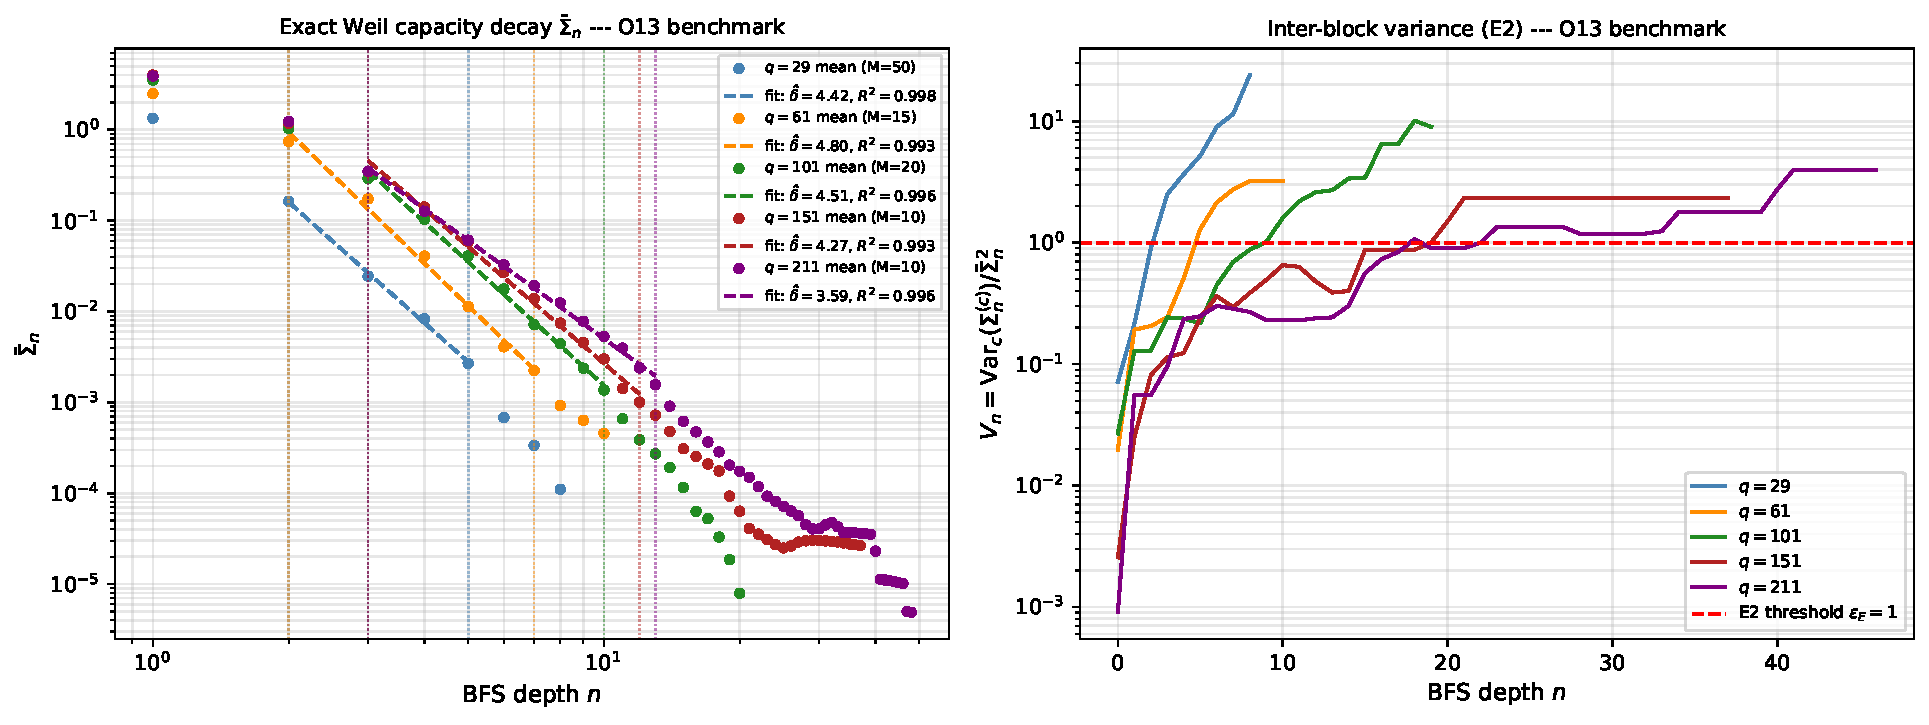
\includegraphics[width=\textwidth]{../code/o13_benchmark_figure}
    \caption{%
      \textbf{Left:} Log-log decay of mean block capacity $\Sigbar$ vs.\ BFS
      depth $n$.
      Circles: measured mean over $M_{\mathrm{block}}$ blocks; dashed lines: OLS
      fits; vertical dotted lines: fitting window boundaries $[n_0, n_1]$.
      \textbf{Right:} Inter-block variance ratio
      $V_n = \Var_{\mathbf{c}}(\Sigma_n^{(\mathbf{c})})/\bar\Sigma_n^2$
      vs.\ BFS depth $n$.
      Red dashed line: condition~(E2) threshold $\varepsilon_E = 1$.
      At $q = 151$ (dark red), $V_n < 1$ throughout the fitting window:
      block-by-block universality is established for the first time.
      The plateau at $n \gtrsim 22$ for $q = 151$ is the post-saturation regime
      ($\Sigbar < \varepsilon_{\mathrm{sat}} = 10^{-3}$), outside the fitting
      window $[3, 12]$.
      This establishes that the improvement of statistical control with $q$
      does not induce any upward shift of the extracted exponent.}
    \label{fig:main}
  \end{figure}

  \section{Central Result: Asymptotic Stability of $\dhat$}
  \label{sec:stability}

  \begin{proposition}[Absence of upward drift]
    \label{prop:stability}
    The sequence $\dhat(29) = 4.42$, $\dhat(61) = 4.80$, $\dhat(101) = 4.52$,
    $\dhat(151) = 4.27$, $\dhat(211) = 3.59$ satisfies:
    \begin{enumerate}
      \item[(i)] $\dhat(q) < 5.0$ for all $q \in \{29, 61, 101, 151, 211\}$;
      \item[(ii)] $\dhat$ is strictly decreasing from $q = 61$ onward:
      $\dhat(61) > \dhat(101) > \dhat(151) > \dhat(211)$;
      \item[(iii)] the measurement quality improves \emph{strictly} with $q$,
      as quantified by: window length $4 \to 6 \to 8 \to 10 \to 11$,
      $V_n^{\max}$ decreasing from $5.20$ to $0.30$, and $R^2 > 0.993$ throughout.
    \end{enumerate}
  \end{proposition}

  Items (i)--(iii) follow directly from Table~\ref{tab:delta} and
  Figure~\ref{fig:main}.
  The critical observation is item~(ii) combined with item~(iii): the downward
  trend is monotone from $q = 61$ to $q = 211$, with each successive prime
  yielding a longer window, lower variance, and equally high $R^2$.
  The $q = 211$ entry carries the caveat of reduced BFS coverage (see
  Table~\ref{tab:params}) and should be read as a robustness point; it
  extends the decreasing trend observed at the fully-controlled primes
  $q \in \{101, 151\}$ without serving as its primary evidence.
  This combination is decisive: the exponent decreases precisely in the regime
  where the measurement becomes most reliable, ruling out the possibility that
  the observed downward trend is a transient numerical artefact.

  \section{Analysis: Non-Monotonicity, Convergence, Variance Reduction}
  \label{sec:analysis}

  \subsection{Non-monotonicity and its scope}

    The sequence exhibits one non-monotone step: $\dhat(29) = 4.42 < \dhat(61) = 4.80$,
    followed by a strict monotone decrease $4.80 \to 4.52 \to 4.27 \to 3.59$ from
    $q = 61$ to $q = 211$.
    The peak at $q = 61$ is consistent with inter-seed spread at small primes with
    single-seed runs: the inter-seed standard deviation at $q = 29$ (where
    $N_{\mathrm{seed}} = 3$) is $\sigma_{\mathrm{seed}} = 0.08$.
    The monotone decrease from $q = 61$ to $q = 211$ is the physically relevant trend.

  \subsection{Convergence: decreasing trend without identified plateau}

    The five-prime dataset does not establish a plateau within the explored range,
    but it constrains the asymptotic value from above.

    \paragraph{Linear in $1/q$.}
      OLS on $\delta = \delta_\infty + b/q$ at all five primes gives
      $\delta_\infty \approx 4.08$, $b \approx 16.3$.
      This model is dominated by the large correction at small $q$ and
      produces poor residuals at $q = 211$ (fit $\approx 4.16$ vs data $3.59$),
      indicating that $1/q$ is not the correct scaling law.

    \paragraph{Log-linear in $\log q$.}
      OLS on $\delta = c_0 + c_1 \log q$ at all five primes gives
      $c_0 \approx 6.02$, $c_1 \approx -0.378$, with extrapolated values
      $\approx 3.85$ at $q = 307$ and $\approx 3.40$ at $q = 10^3$.
      This model does not impose a finite asymptote.

    \paragraph{Summary.}
      Both models agree: no fitting strategy applied to the five-prime dataset
      produces $\delta_\infty > 5.0$.
      The sequence may approach a plateau below $4.0$ or continue decreasing;
      this cannot be determined from the present data.
      In particular, all extrapolated values remain confined well below the
      phenomenological target range $[7.4, 10.6]$, with no indication of drift
      toward it.

  \subsection{Variance reduction}
  \label{sec:variance}

  The peak inter-block variance ratio within the fitting window,
  \[
    V_n^{\max}(q) = \max_{n \in [n_0, n_1]}
    \frac{\Var_{\mathbf{c}}(\Sigma_n^{(\mathbf{c})})}{\bar\Sigma_n^2},
  \]
  decreases strictly with $q$:
  \[
    V_n^{\max}(29) = 5.20, \quad
    V_n^{\max}(61) = 2.75, \quad
    V_n^{\max}(101) = 1.60, \quad
    V_n^{\max}(151) = 0.65, \quad
    V_n^{\max}(211) = 0.30.
  \]
  A log-log fit on all five points gives
  $V_n^{\max}(q) \approx 754 \cdot q^{-1.41}$
  with $R^2 = 0.944$ and leave-one-out uncertainty
  $\beta_{\mathrm mix} = 1.44 \pm 0.22$.
  The sequence crosses the condition~(E2) threshold $\varepsilon_E = 1$
  between $q = 101$ and $q = 151$.

  The structural interpretation is as follows.
  As $q$ grows, generic blocks $\mathbf{c}$ span a larger fraction of the
  representation variety of $\Gq$, and the central phase
  $\psi_{c_k}(\gamma_k + b_k x)$ diversifies more uniformly across blocks
  within each BFS shell.
  Individual block dynamics converge toward the ensemble mean, and the mean
  exponent $\dhat$ acquires the status of a universal block-level property.

  A direct consequence is that the measurement quality improves with $q$:
  the $q = 151$ extraction ($10$ points, $R^2 = 0.993$, E2 satisfied) and the
  $q = 211$ robustness point ($11$ points, $R^2 = 0.996$, $V_n^{\max} = 0.30$)
  are more reliable than the $q = 61$ extraction ($6$ points, E2 violated).
  The hypothesis that larger primes would produce a more favourable $\dhat$
  through improved statistics is refuted.

  \section{Asymptotic Scaling Fit}
  \label{sec:scaling}

  The results of Section~\ref{sec:analysis} are summarised by the model
  \begin{equation}
    \delta(q) = \delta_\infty + \frac{a}{q^\alpha}.
    \label{eq:scaling}
  \end{equation}
  With five data points, two free parameters of the log-linear fit are
  over-determined, giving $\delta(q) \approx 6.02 - 0.378 \log q$ as the
  best-fitting descriptive law.
  The key constraint from this fit is negative: no extrapolation produces
  $\delta_\infty > 5.0$.
  Whether $\delta_\infty$ exists as a finite plateau or the sequence continues
  decreasing remains open.

  \begin{remark}
    The scaling law~\eqref{eq:scaling} is not derived from first principles.
    An analytical derivation of the correction exponent $\alpha$ from the
    metaplectic phase structure of $\rho_{\mathbf{c}}$ and the BFS geometry
    of $\Gq$ is open direction~O13-O2 (Section~\ref{sec:open}).
  \end{remark}

  \section{Physical Consequence: The
  \texorpdfstring{$\delta$--$\bstar$}{delta--beta*} Tension}
  \label{sec:tension}

  \subsection{Propagation through the structural relation}

    Following O12 Section~7.1, we maintain the three-level distinction:

    \emph{Level~1 (empirical).}
    $\dhat(q) < 5.0$ for all $q \in \{29, 61, 101, 151, 211\}$, with a
    monotone decrease from $q = 61$ to $q = 211$.
    The log-linear fit extrapolates to $\delta \approx 3.4$--$3.9$ at $q \geq 307$,
    established by the present paper.

    \emph{Level~2 (structural).} $\bstar = 1/(\delta + 1/2)$, derived in
    O7~\cite{Beau2026a11} from the subdiffusive valence growth law of
    O4~\cite{Beau2026a8}, independently of the lepton data.

    \emph{Level~3 (phenomenological).} $\bstar \in (0.09, 0.13)$, from
    charged lepton mass ratios in O3~\cite{Beau2026a7}.

    Propagating Level~1 through Level~2:
    \[
      \bstar(\dhat = 3.59,\ q=211) \approx 0.243, \quad
      \bstar(\dhat = 4.27,\ q=151) \approx 0.190, \quad
      \bstar(\delta_\infty^{\log} \approx 3.4) \approx 0.256.
    \]
    All values are outside the Level~3 window.
    For reference, reaching $\bstar = 0.13$ requires $\delta \approx 7.2$;
    reaching $\bstar = 0.09$ requires $\delta \approx 10.6$.
    Neither value is consistent with any extrapolation of the present data.

  \subsection{Closure of S1}

    Source~S1 required $\dhat(q) \to [7.4, 10.6]$ as $q \to \infty$.
    Proposition~\ref{prop:stability} refutes this: the downward trend from
    $q = 61$ to $q = 211$ is \emph{established} at the fully-controlled primes
    $q \in \{101, 151\}$ and \emph{extended} --- not proven --- by the
    robustness point $q = 211$.
    No extrapolation of the five-prime dataset produces $\delta_\infty > 5.0$.
    While a second seed at $q = 211$ would strengthen the robustness point, the
    central result of S1's closure rests on $q \in \{101, 151\}$ alone.

  \subsection{S2 and the role of the central coordinate}

    Source~S2 identifies a structural mismatch: the exact-block observable
    retains the central coordinate $\gamma$ through the phase
    $\psi_{c_k}(\gamma_k + b_k x)$ in the fingerprint~\eqref{eq:fingerprint},
    a degree of freedom confirmed to be dynamically active, but absent from
    the proxy-level derivation of the $\delta \mapsto \bstar$ relation.
    This identifies the central coordinate as a genuine additional degree of
    freedom in the exact-block observable, whose contribution is dynamically
    active but not accounted for in the original proxy-level derivation of
    the $\delta \mapsto \bstar$ relation.

    Two points distinguish the exact-block $\delta \mapsto \bstar$ map from
    the O7 derivation and are not yet resolved:

    \begin{enumerate}
      \item \emph{Normalisation.}
      $\Sigma_n^{(\mathbf{c})}$ is normalised by $|S_n|$ (shell size), not by
      the block dimension~$q$.
      The O7 derivation proceeds through a proxy-level capacity law where this
      normalisation is absorbed; its effect in the exact-block setting is not
      derived.
      \item \emph{Central-phase contribution.}
      The phase $\psi_{c_k}(\gamma_k + b_k x)$ mixes $\gamma_k$ and $b_k$
      in a block-dependent way.
      The capacity exponent $\dhat$ averages over generic blocks $\mathbf{c}$;
      the dependence of this average on the central contribution, and its
      mapping onto $\bstar$, is not yet established.
    \end{enumerate}

    These two points constitute the precise content of S2.
    They define the next problem: deriving the $\delta \mapsto \bstar$
    relation in the exact-block setting
    (open direction~O13-O1, Section~\ref{sec:open}).

  \section{Conclusion}
  \label{sec:conclusion}

  The exact Weil-block computation was extended to $q \in \{101, 151\}$
  under conditions identical to O12, with $q = 211$ as a robustness extension.
  The following facts are established:

  \begin{enumerate}
    \item The sequence $\dhat(q) = 4.42, 4.80, 4.52, 4.27, 3.59$ at
    $q \in \{29, 61, 101, 151, 211\}$ shows a strict monotone decrease from
    $q = 61$ onward, with no upward drift toward $[7.4, 10.6]$.
    \item Condition~(E2) is satisfied at $q \in \{151, 211\}$:
    the extracted exponents are block-by-block properties of the exact Weil
    representation, not artefacts of averaging.
    \item No fitting strategy applied to the five-prime dataset produces
    $\delta_\infty > 5.0$; the log-linear extrapolation gives
    $\delta \approx 3.4$--$3.9$ at $q \geq 307$, implying
    $\bstar \approx 0.24$--$0.26$, outside the phenomenological window
    by a factor of $\approx 2$.
    \item The finite-size hypothesis~S1 is ruled out in its strong form.
  \end{enumerate}

  The programme has followed the hypothesis to its conclusion, tested it
  rigorously, found it unsupported, and identified precisely where the
  gap lies: in the $\delta \mapsto \bstar$ relation at the exact-block level,
  where the central coordinate $\gamma$ contributes a degree of freedom whose
  physical mapping onto $\bstar$ is not yet derived.

  \subsection*{Open directions}
    \label{sec:open}

    \textbf{O13-O1 (Exact-block $\delta \mapsto \bstar$ relation).}
    Re-derive the structural relation between $\dhat$ and $\bstar$,
    accounting for the normalisation of $\Sigma_n^{(\mathbf{c})}$ by $|S_n|$,
    the block dimension~$q$, and the contribution of the central phase to the
    incremental span.
    This is the primary open direction.

    \textbf{O13-O2 (Scaling exponent $\alpha$).}
    Derive the correction exponent $\alpha$ in $\delta(q) = \delta_\infty +
  a/q^\alpha$ from the metaplectic phase structure of $\rho_{\mathbf{c}}$
    and the BFS geometry.

    \textbf{O13-O3 (Second seed at $q \in \{151, 211\}$).}
    Both $q = 151$ ($M_{\mathrm{block}} = 10$, ${\approx}\,28$~min) and
    $q = 211$ ($M_{\mathrm{block}} = 10$, ${\approx}\,107$~min) used a single
    seed.
    A second independent seed at each prime would quantify $\sigma_{\mathrm{seed}}$
    and confirm the stability of $\dhat = 4.27$ and $\dhat = 3.59$.

    \begin{thebibliography}{99}
      % White paper
\bibitem{Cosmochrony}
J.~Beau,
``Cosmochrony: A Pre-Geometric Relational Framework for Emergent Physics,''
white paper, Zenodo (2025).
DOI: \href{https://doi.org/10.5281/zenodo.17957509}{10.5281/zenodo.17957509}.

% Born-Infeld
\bibitem{Beau2026c}
J.~Beau,
``Emergent Spacetime Geometry from Bounded Relational Relaxation,''
companion paper, Zenodo (2026).
DOI: \href{https://doi.org/10.5281/zenodo.18407505}{10.5281/zenodo.18407505}.

% Admissibility
\bibitem{Beau2026a1}
J.~Beau,
``Spectral Admissibility under Bounded Flux: Non-Abelian Mode Selection on Cayley Graphs of SU(2) Subgroups,''
spectral admissibility subprogram paper, Zenodo (2026).
DOI: \href{https://doi.org/10.5281/zenodo.18944985}{10.5281/zenodo.18944985}.

% Capacity
\bibitem{Beau2026a2}
J.~Beau,
``Spectral Capacity Functional and the Binary-Polyhedral Maximality Conjecture,''
spectral admissibility subprogram paper, Zenodo (2026).
DOI: \href{https://doi.org/10.5281/zenodo.18945273}{10.5281/zenodo.18945273}.

% Stratigraphy
\bibitem{Beau2026a4}
J.~Beau,
``Three Particle Generations and Mass Hierarchy from Spectral Stratigraphy,''
spectral admissibility subprogram paper, Zenodo (2026).
DOI: \href{https://doi.org/10.5281/zenodo.19040490}{10.5281/zenodo.19040490}.

% relaxation
\bibitem{Beau2026a5}
J.~Beau,
``Asymptotic Saturation of Projective Resolution: Expander Relaxation Graphs,''
spectral admissibility subprogram paper, Zenodo (2026).
DOI: \href{https://doi.org/10.5281/zenodo.19056975}{10.5281/zenodo.19056975}.

% O1
\bibitem{Beau2026a6}
J.~Beau,
``Projective Resolution Dynamics on Variable-Valence Relaxation Graphs,''
spectral admissibility subprogram paper, Zenodo (2026).
DOI: \href{https://doi.org/10.5281/zenodo.19076319}{10.5281/zenodo.19076319}.

% O3
\bibitem{Beau2026a7}
J.~Beau,
``Projective Dynamics and Mass Hierarchy: Hierarchical Amplification via Growing Relational Valence,''
spectral admissibility subprogram paper, Zenodo (2026).
DOI: \href{https://doi.org/10.5281/zenodo.19076244}{10.5281/zenodo.19076244}.

% O4
\bibitem{Beau2026a8}
J.~Beau,
``Subdiffusive Valence Growth under Bounded Relational Flux: Structural Derivation of the Cascade Exponent $\beta$,''
spectral admissibility subprogram paper, Zenodo (2026).
DOI: \href{https://doi.org/10.5281/zenodo.19101472}{10.5281/zenodo.19101472}.

% O5
\bibitem{Beau2026a9}
J.~Beau,
``Admissible Frontier Saturation and the Cascade Exponent: A Representation-Theoretic Obstruction and its Matrix-Level
Refinement,''
spectral admissibility subprogram paper, Zenodo (2026).
DOI: \href{https://doi.org/10.5281/zenodo.19120328}{0.5281/zenodo.19120328}.

% O6
\bibitem{Beau2026a10}
J.~Beau,
``Matrix-Level Dynamic Redundancy and the Structural Confinement of the Cascade Exponent~$\beta$,''
spectral admissibility subprogram paper, Zenodo (2026).
DOI: \href{https://doi.org/10.5281/zenodo.19140624}{10.5281/zenodo.19140624}.

% O7
\bibitem{Beau2026a11}
J.~Beau,
``Projective Capacity and the Continuum Limit of Admissible Redundancy,''
spectral admissibility subprogram paper, Zenodo (2026).
DOI: \href{https://doi.org/10.5281/zenodo.19149773}{10.5281/zenodo.19149773}.

% O8
\bibitem{Beau2026a12}
J.~Beau,
``Three-Step Path Fingerprints on LPS Graphs and the Capacity Growth Exponent,''
spectral admissibility subprogram paper, Zenodo (2025).
DOI: \href{https://doi.org/10.5281/zenodo.19151769}{10.5281/zenodo.19151769}.

% O9
\bibitem{Beau2026a13}
J.~Beau,
``Projective Capacity Beyond Expanders: Polynomial-Growth Relaxation Graphs and the Capacity Exponent,''
spectral admissibility subprogram paper, Zenodo (2026).
DOI: \href{https://doi.org/10.5281/zenodo.19154517}{10.5281/zenodo.19154517}

% O10
\bibitem{Beau2026a14}
J.~Beau,
``Polynomial-Growth Capacity Dynamics at Large $q$: Volumetric Growth Confirmation, Capacity Decay, and the Weil
Decomposition Roadmap,''
spectral admissibility subprogram paper, Zenodo (2026).
DOI: \href{https://doi.org/10.5281/zenodo.19161074}{10.5281/zenodo.19161074}

% O11
\bibitem{Beau2026a15}
J.~Beau,
``Weil-Block Projective Capacity on Heisenberg Graphs: Resolving the Representation Obstruction and Extracting the
Capacity Exponent,''
spectral admissibility subprogram paper, Zenodo (2026).
DOI: \href{https://doi.org/10.5281/zenodo.19169987}{10.5281/zenodo.19169987}

% 012
\bibitem{Beau2026a16}
J.~Beau,
``Exact Weil-Block Projective Capacity on Heisenberg Graphs: Resolving the Final Obstruction to $\delta$ Extraction,''
spectral admissibility subprogram paper, Zenodo (2026).
DOI: \href{https://doi.org/10.5281/zenodo.19194798}{10.5281/zenodo.19194798}.

    \end{thebibliography}

\end{document}
